\section{Auswertung}
\label{sec:Auswertung}
Ziel der Auswertung ist das Bestimmen der Spaltbreite $b_i$ und ein anschließender Vergleich mit der Herstellerangabe.
Für den Versuch werden alle zur Verfügung stehenden Randdaten in Tabelle \ref{tab:rand} dokumentiert.

\begin{table}
    \centering
    \caption{Kenndaten der Versuchsdurchführung.}
    \label{tab:rand}
    \begin{tabular}{c c c c c c c}
        \toprule
        & $s\:/\:\si{\milli\meter}$ & $b_i\:/\:\si{\milli\meter}$ & $\lambda\:/\:\si{\nano\meter}$ & $d\:/\:\si{\milli\meter}$ & $I_d\:/\:\si{\micro\ampere}$ \\
        \midrule
        Einzelspalt &      & 0.075 & 633 & 626.1 & 0.70 \\
        Doppelspalt & 0.75 & 0.150 & 633 & 626.1 & 0.63 \\
        \bottomrule
    \end{tabular}
\end{table}

\subsection{Einzelspalt}

\begin{table}
    \centering
    \caption{Messwerte zum Einzelspalt.}
    \label{tab:Mess1}
    \begin{tabular}{S[table-format=1.1] S[table-format=1.3] S[table-format=2.2] S[table-format=1.1] S[table-format=1.3] S[table-format=2.2] S[table-format=1.1] S[table-format=1.3]}
        \toprule
        $x\:/\:\si{\milli\meter}$ & $I\:/\:\si{\micro\ampere}$ &&
        $x\:/\:\si{\milli\meter}$ & $I\:/\:\si{\micro\ampere}$ &&
        $x\:/\:\si{\milli\meter}$ & $I\:/\:\si{\micro\ampere}$ \\
        \midrule
        0.0 & 0.880 && 8.5   & 3.300  && 17.0 & 0.865 \\
        0.5 & 0.840 && 9.0   & 5.000  && 17.5 & 0.990 \\
        1.0 & 0.778 && 9.5   & 7.000  && 18.0 & 1.150 \\
        1.5 & 0.740 && 10.0  & 9.000  && 18.5 & 1.260 \\
        2.0 & 0.758 && 10.5  & 10.700 && 19.0 & 1.290 \\
        2.5 & 0.854 && 11.0  & 12.100 && 19.5 & 1.220 \\
        3.0 & 1.000 && 11.5  & 12.700 && 20.0 & 1.100 \\
        3.5 & 1.200 && 12.0  & 12.700 && 20.5 & 0.975 \\
        4.0 & 1.340 && 12.5  & 12.250 && 21.0 & 0.880 \\
        4.5 & 1.430 && 13.0  & 10.600 && 21.5 & 0.842 \\
        5.0 & 1.400 && 13.5  & 8.850  && 22.0 & 0.879 \\
        5.5 & 1.250 && 14.0  & 6.790  && 22.5 & 0.945 \\
        6.0 & 1.050 && 14.5  & 4.780  && 23.0 & 1.000 \\
        6.5 & 0.900 && 15.0  & 3.000  && 23.5 & 1.060 \\
        7.0 & 0.910 && 15.5  & 1.920  && 24.0 & 1.070 \\
        7.5 & 1.260 && 16.0  & 1.200  && 24.5 & 1.025 \\
        8.0 & 2.040 && 16.5  & 0.890  &&      &       \\
        \bottomrule
    \end{tabular}
\end{table}

Für die Ausgleichskurve des Einzelspalts wird eine an \ref{eqn:I} angelehnte Funktion der Form
\begin{equation}
    I(\varphi) = (a\frac{\sin{\gamma}}{\gamma})^2 + c
    \label{eqn:Iaus}
\end{equation}
verwendet\footnote{In der Diskussion \ref{sec:Erweiterte Diskussion} wird diese Form weiter diskutiert.} mit 
\begin{equation}
    \gamma = \frac{\pi b_{par, 1} \sin\varphi}{\lambda}
    \label{eqn:gamma}
\end{equation}
\begin{equation}
    \sin\varphi = \frac{x'}{d'}
\end{equation}
\begin{equation}
    d' = \sqrt{d^2 + x'^2}
\end{equation}
und
\begin{equation}
    x' = |x - x_0| \:.
\end{equation}
Die variablen Parameter der Funktion sind $x_0$, $a$, $b_{par, 1}$, und $c$, wobei $x_0$ das Intensitätsmaximum, $a$ das $A_0$ aus \eqref{eqn:I}, $b_{par, 1}$ die Spaltbreite und $c$ der Dunkelstrom
$I_d$ ist.
Die Ausgleichsrechnung mit der Funktion mit \texttt{curve\_fit}\cite{scipy} liefert die Werte in Tabelle \ref{tab:parEinzel}.

\begin{table}
    \centering
    \caption{Parameterwerte des Einzelspalts.}
    \label{tab:parEinzel}
    \begin{tabular}{c S[table-format=1.6]@{\,\( \pm \)\,}S[table-format=1.6] 
        S[table-format=1.5]@{\,\( \pm \)\,}S[table-format=1.5] 
        S[table-format=1.2]@{\,\( \pm \)\,}S[table-format=1.2]
        S[table-format=1.3]@{\,\( \pm \)\,}S[table-format=1.3]}
        \toprule
        & \multicolumn{2}{c}{$a$} & \multicolumn{2}{c}{$b_{par, 1}\:/\:\si{\milli\meter}$} & \multicolumn{2}{c}{$c\:/\:\si{\micro\ampere}$} & \multicolumn{2}{c}{$x_0\:/\:\si{\milli\meter}$} \\
        \midrule
        Einzelspalt & 0.003481&0.000005 & 0.0784&0.0002 & 0.81&0.01 & 11.727&0.006 \\
    \end{tabular}
\end{table}
Die Herstellerangabe $b_{1} = \SI{0.075}{\milli\meter}$ ist mit dem errechneten Wert für die Spaltbreite um $\Delta b_{par, 1} \approx \SI{0.0034}{\milli\meter}$ und damit um etwa $4.5\%$ verschieden. 
Die relative Messunsicherheit von $b_{par, 1}$ ist $\approx 2.5\%$.

\begin{figure}
    \centering
    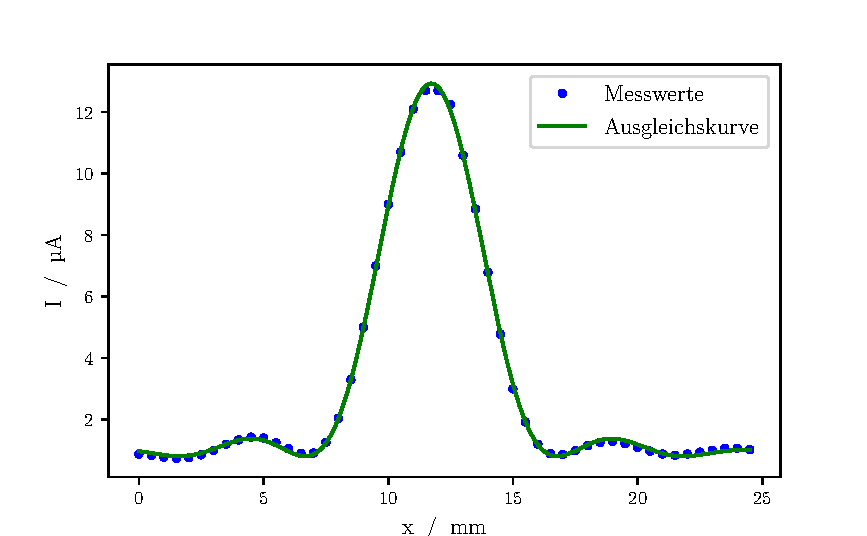
\includegraphics[width=.9\textwidth]{python/EinzelspaltFit.pdf}
    \caption{Messwerte und Ausgleichskurve zum Einzelspalt.}
    \label{fig:messEinzel}
\end{figure}

Der abgeschätzte Wert des Intensitätsmaximums $x_0$ liegt bei $\SI{11.727 \pm 0.008}{\milli\meter}$ mit einer Unsicherheit von $0.07\%$.

\subsection{Doppelspalt}
\begin{table}
    \centering
    \caption{Parameterwerte des Doppelspalts.}
    \label{tab:parDoppel}
    \begin{tabular}{S[table-format=1.5]@{\,\( \pm \)\,}S[table-format=1.5] 
        S[table-format=1.4]@{\,\( \pm \)\,}S[table-format=1.4] 
        S[table-format=1.1]@{\,\( \pm \)\,}S[table-format=1.1]
        S[table-format=1.3]@{\,\( \pm \)\,}S[table-format=1.3]
        S[table-format=1.3]@{\,\( \pm \)\,}S[table-format=1.3]}
        \toprule
        \multicolumn{2}{c}{$a$} & \multicolumn{2}{c}{$b_{par, 2}\:/\:\si{\milli\meter}$} & \multicolumn{2}{c}{$c\:/\:\si{\micro\ampere}$} & \multicolumn{2}{c}{$x_0\:/\:\si{\milli\meter}$} & \multicolumn{2}{c}{$s\:/\:\si{\milli\meter}$}\\
        \midrule
        0.00454&0.00001 & 0.147&0.001 & 0.8&0.1 & 11.077&0.005 & 0.021&0.003\\
    \end{tabular}
\end{table}

\begin{table}
    \centering
        \caption{Messwerte zum Doppelspalt.}
        \label{tab:Mess2}
        \begin{tabular}{S[table-format=1.1] S[table-format=1.3] S[table-format=2.2] S[table-format=1.1] S[table-format=1.3] S[table-format=2.2] S[table-format=1.1] S[table-format=1.3]}
            \toprule
            $x\:/\:\si{\milli\meter}$ & $I\:/\:\si{\micro\ampere}$ &&
            $x\:/\:\si{\milli\meter}$ & $I\:/\:\si{\micro\ampere}$ &&
            $x\:/\:\si{\milli\meter}$ & $I\:/\:\si{\micro\ampere}$ \\
            \midrule
            0.00 & 0.942 && 7.99  & 2.420  && 15.98 & 0.800 \\
            0.47 & 0.920 && 8.46  & 1.300  && 16.45 & 0.960 \\
            0.94 & 0.718 && 8.93  & 4.350  && 16.92 & 1.380 \\
            1.41 & 0.620 && 9.40  & 15.800 && 17.39 & 1.430 \\
            1.88 & 0.724 && 9.87  & 42.400 && 17.86 & 1.030 \\
            2.35 & 0.910 && 10.34 & 63.000 && 18.33 & 0.710 \\
            2.82 & 0.936 && 10.81 & 80.000 && 18.80 & 0.730 \\
            3.29 & 0.750 && 11.28 & 81.800 && 19.27 & 0.940 \\
            3.76 & 0.635 && 11.75 & 67.500 && 19.74 & 1.050 \\
            4.23 & 0.810 && 12.22 & 42.500 && 20.21 & 0.840 \\
            4.70 & 1.120 && 12.69 & 20.400 && 20.68 & 0.665 \\
            5.17 & 1.140 && 13.16 & 6.350  && 21.15 & 0.685 \\
            5.64 & 1.070 && 13.63 & 1.430  && 21.62 & 0.855 \\
            6.11 & 0.720 && 14.10 & 1.880  && 22.09 & 0.980 \\
            6.58 & 1.445 && 14.57 & 2.950  && 22.56 & 0.900 \\
            7.05 & 2.850 && 15.04 & 2.740  && 23.03 & 0.715 \\
            7.52 & 3.450 && 15.51 & 1.540  &&       &       \\
            \bottomrule
        \end{tabular}
\end{table}

Für den Doppelspalt wird die angepasste Funktion \eqref{eqn:doppelspalt} verwendet. Dabei entspricht das $\gamma$ dem aus \eqref{eqn:gamma}.

Als Kontrollwert der Parameter für den Doppelspalt eignet sich $x_0 = \SI{11.077 \pm 0.005}{\milli\meter}$, welcher eine gute und plausible Annäherung an das gemessene Intensitätsmaximum ist. (Vgl. Tab. \ref{tab:Mess2} und Abb. \ref{fig:messDoppel})
\begin{figure}
    \centering
    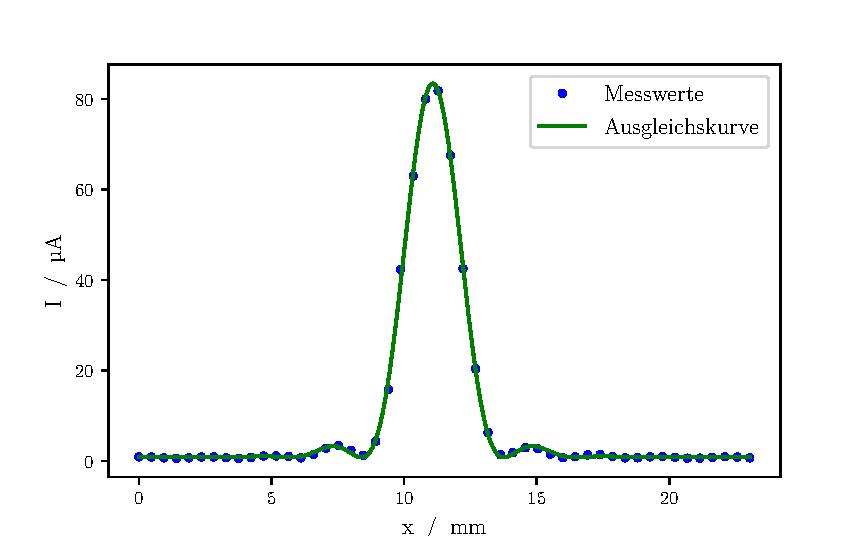
\includegraphics[width=.9\textwidth]{python/DoppelspaltFit.pdf}
    \caption{Messwerte und Ausgleichskurve zum Doppelspalt.}
    \label{fig:messDoppel}
\end{figure}

Die Herstellerangabe zur Spaltbreite $b_2 = \SI{0.15}{\milli\meter}$ ist dem ermittelten Wert $b_{par, 2} = \SI{0.147 \pm 0.001}{\milli\meter}$
um ungefähr $\Delta b_{par, 2} = \SI{0.003}{\milli\meter}$ verschieden. Das entspricht einer Abweichung von $2\%$.

Die relative Messunsicherheit von $b_{par, 2}$ ist $\approx 0.6\%$.

Für den Spaltabstand weicht der errechnete Wert $s = \SI{0.021 \pm 0.003}{\milli\meter} \approx \SI{0.02}{\milli\meter}$ um den Faktor $35.7$ von der Herstellerangabe $s_H = \SI{0.75}{\milli\meter}$ ab.

\subsection{Erweiterte Auswertung}
Die große Abweichung und die möglichen Ursachen werden in der erweiterten Diskussion \ref{sec:Erweiterte Diskussion} thematisiert.
Im weiteren Verlauf wird die Methodik der Ausgleichsrechnung sowie alternative Parameter ausgewertet. Der folgende Abschnitt geht also ein wenig über die ursprüngliche
Thematik hinaus und beleuchtet einen sonst für selbstverständlich angenommenen Aspekt.\\

\subsubsection{Einschub: Methode der kleinsten Quadrate}
Das Berechnen der optimalen Parameter erfolgt über die \textit{Methode der kleinsten Quadrate}, bei der das Minimum der Fehlerquadratsummen gesucht wird.
Hierbei ist beispielsweise $\vec{\beta} = (\beta_1, \beta_2, ..., \beta_m),\:\vec{\beta}\in\mathbb{R}^m$ die Menge aller Parameter.
Die Summe berechnet sich dann über
\begin{equation}
    S = \sum_i^n (y_i - f(x_i, \vec{\beta}))^2 \:.
    \label{eqn:fehlerquadratsumme}
\end{equation}
Die Menge aller Wertepaare $[(x_i, y_i)],\: i\in[0, 1, ..., n]$ stellt die Messdaten dar. Die Funktion $f$ stammt aus demjenigen Modell, von dem das Verhalten
der Messwere vermutet wird.
In diesem Falle sind das die Funktionen des Einzel- \eqref{eqn:I} und des Doppelspalts \eqref{eqn:doppelspalt}.
Für das Minimum werden also die Parameter
\begin{equation}
    \min\limits_{\vec{\beta}} \sum_i^n (y_i - f(x_i, \vec{\beta}))^2
\end{equation}
gesucht. Für den Einzelspalt sind das die Parameter $a, b$
\begin{equation}
    \min\limits_{a, b} \sum_i^n (y_i - f(x_i, a, b))^2 \:.
\end{equation}

\subsubsection{Parameterebenen}
Im folgenden werden die Parameter-Wertepaare $[(a_i,b_i)],\:i\in[0,1,..,m]$ als Ebene dargestellt.
Jedes Wertepaar besitzt eine (positive) Fehlerquadratsumme, sodass die resultierende Ebene nach Minima untersucht werden kann.

\textbf{Ziel der Ebenendarstellung} ist das Aufdecken möglicher Minima, die relativ nah beieinander liegen.
Auf diese Weise wird überprüft, ob es plausible Parameter gibt (näher an den Herstellerangaben), für die die Ausgleichskurve zwar nicht optimal,
aber dennoch hinreichend genau ist.

\textbf{Erwartung:} Wellenartige Ebene mit tropfenförmigen Senken, an denen die Parameter lokal gegen ein Minimum konvergieren. Das Minimum der Fehlerquadratsummen kann analytisch über
das Nullsetzen der partiellen Ableitungen nach den Parametern, hier $\partial a$ und $\partial b$, bestimmt werden.
Daher erzeugen periodische Funktionen auch periodische Parameterebenen.

\subsubsection{Einzelspalt}
Die in Tabelle \ref{tab:parEinzel} berechneten, additiven Konstanten $x_0 = \SI{11.727}{\milli\meter}$ und $I_d = \SI{0.8}{\nano\ampere}$ werden festgesetzt,
damit die Funktion \eqref{eqn:I} $f:(x,a,b)\mapsto y$ abgesehen von $x$ nur noch von den Parametern $(a,b)$ abhängt.
Anschließend wird die Fehlerquadratsumme für bestimmte Intervalle $(a_{min}, a_{max})$ und $(b_{min}, b_{max})$ berechnet und in einer Matrix $C = mat(1000, 1000)$ eingetragen.
Jeder Matrixeintrag entspricht einem anderen Parameter-Wertepaar.
Eine Parameterebene mit weit gefassten Intervallen ist in \ref{fig:ls1} zu sehen.
Für alle Ebenen ist $n = 1000$ ($n$ Schritte im Intervall).

\begin{figure}
    \centering
    \textbf{Parameterebene Einzelspalt - große Intervalle.}\par\medskip
    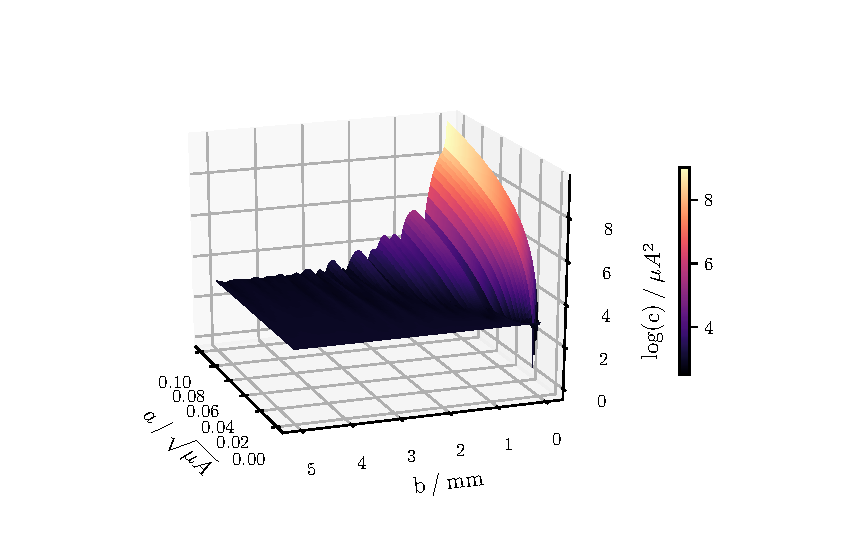
\includegraphics[width=.9\textwidth]{python/leastSquares.pdf}
    \caption{$a = (0.00001, 0.1)$, $b = (0.0001, 5)$.}
    \label{fig:ls1}
\end{figure}

Die Ebene ist wie erwartet wellenförmig, jedoch konvergieren die Parameterwerte nur in einem sehr, sehr kleinen Bereich zu einem Minimum, nahe der Null.

\begin{figure}
    \centering
    \textbf{Parameterebene Einzelspalt.}\par\medskip
    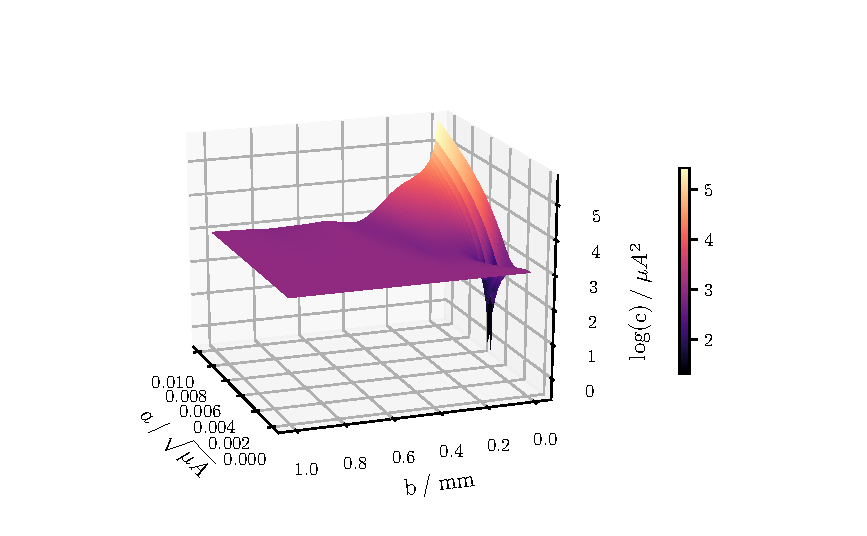
\includegraphics[width=.9\textwidth]{python/leastSquares2.pdf}
    \caption{$a = (0.00001, 0.01)$, $b = (0.0001, 1)$.}
    \label{fig:ls2}
\end{figure}

Die weiteren Abbildungen \ref{fig:ls2}, \ref{fig:ls3} und \ref{fig:ls4} zeigen jeweils einen vergrößerten Ausschnitt des Minimums.
Abbildung \ref{fig:2d} zeigt eine alternative, 2-Dimensionale Darstellung.

%\centering %das war vermutlich der Fehler ;) RL: jop.
\begin{figure}
    \centering
    \textbf{Parameterebene Einzelspalt.}\par\medskip
    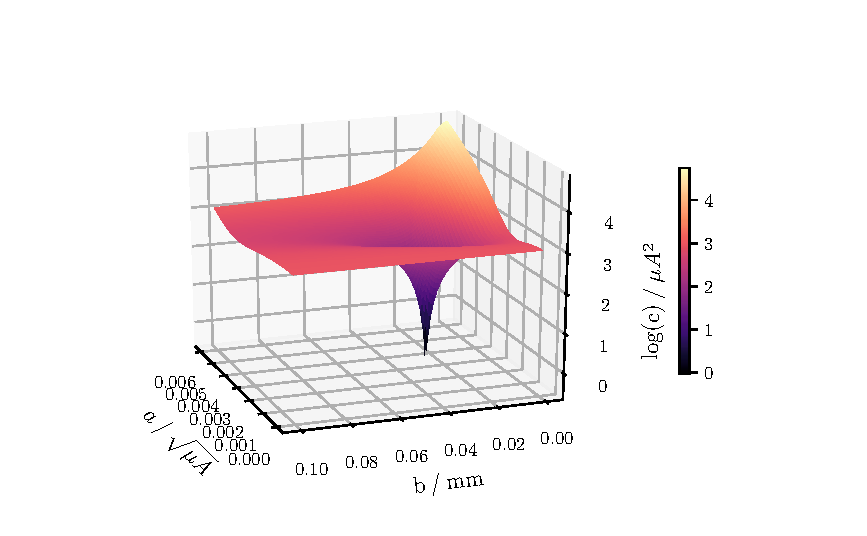
\includegraphics[width=.9\textwidth]{python/leastSquares3.pdf}
    \caption{$a = (0.00001, 0.006)$, $b = (0.0001, 0.1)$\footnote{Herstellerangabe $b=\SI{0.075}{\milli\meter}$}.}
    \label{fig:ls3}
\end{figure}

\begin{figure}
    \centering
    \textbf{Parameterebene Einzelspalt - maximale Vergößerung.}\par\medskip
    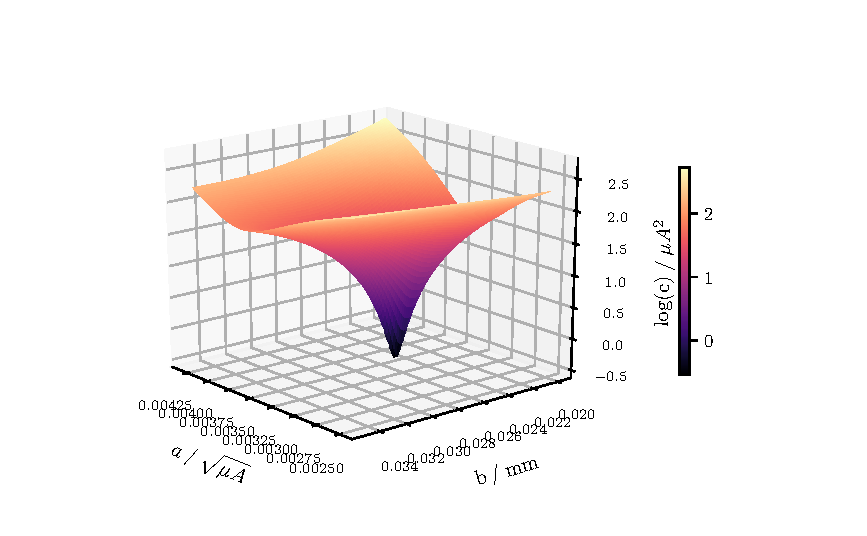
\includegraphics[width=.9\textwidth]{python/leastSquares5.pdf}
    \caption{$a = (0.0025, 0.0043)$, $b = (0.02, 0.035)$.}
    \label{fig:ls4}
\end{figure}


\begin{figure}
    \centering
    \textbf{Einzelspalt - Kurvenschar.}\par\medskip
    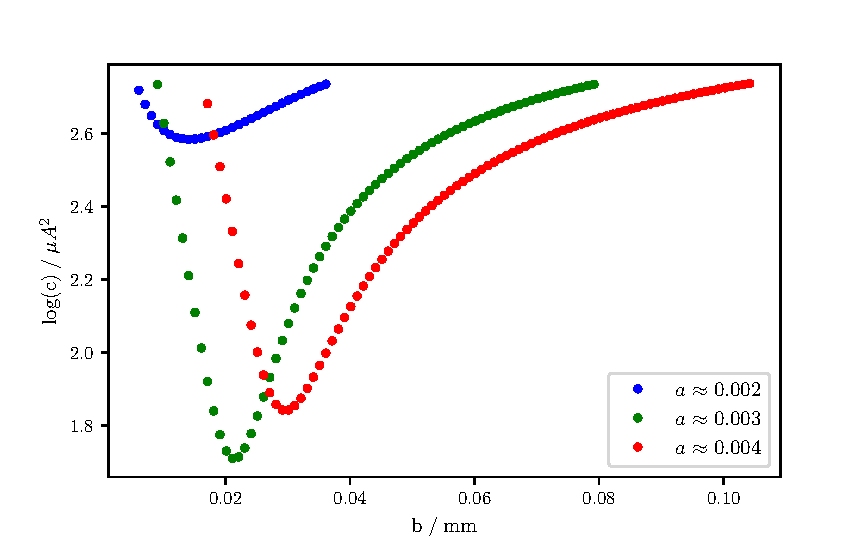
\includegraphics[width=.9\textwidth]{python/2DPlot.pdf}
    \caption{Kurvenschar der Fehlerquadratsumme in Abhängigkeit von $a$ und $b$.}
    \label{fig:2d}
\end{figure}

\subsubsection{Doppelspalt}
Die Parameterebene wird nach demselben Prinzip erstellt, jedoch wird die Funktion um einen Parameter $s$ erweitert. Dadurch ist die
Fehlerquadratsumme geometrisch schwieriger darzustellen.
Für eine Gegenüberstellung wird der Parameter $s$ konstant gehalten. Es werden zwei Fälle unterschieden:\\
\begin{enumerate}
    \item Für $s$ wird die Herstellerangabe verwendet.
    \item Für $s$ wird der optimale Parameterwert aus \texttt{curve\_fit} verwendet.
\end{enumerate}
Hierdurch können die Parameterebenen sowohl auf lokale Minima, als auch auf Verschiebungen dieser Minima durch den Parameterwechsel in $s$
untersucht werden.

\begin{figure}
    \centering
    \textbf{Parameterebene Doppelspalt - fester Spaltabstand}\par\medskip
    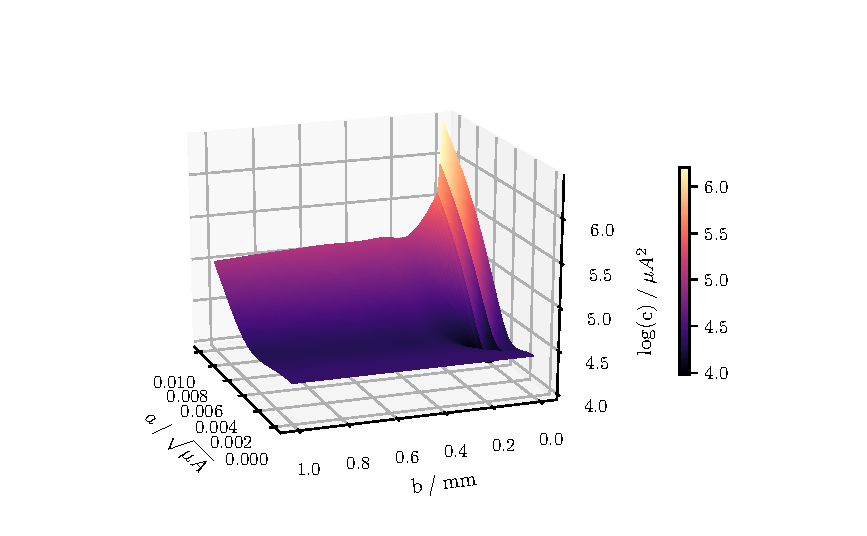
\includegraphics[width=.9\textwidth]{python/leastSquaresDoppel2ss.pdf}
    \caption{$s = \SI{0.75}{\milli\meter}$ (Herstellerangabe), $a = (0.00001, 0.01)$, $b = (0.0001, 1)$.}
    \label{fig:lsd2ss}
\end{figure}
\begin{figure}
    \centering
    \textbf{Parameterebene Doppelspalt - bester Fit, dynamische Parameter}\par\medskip
    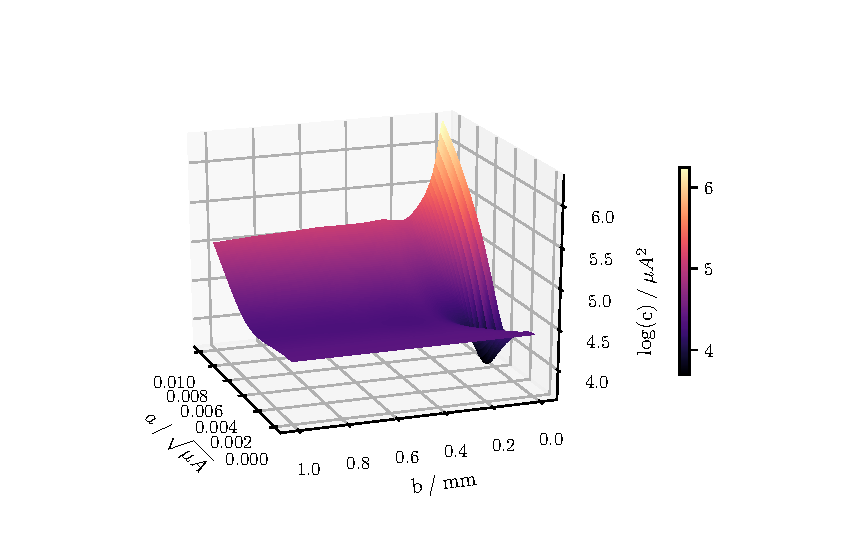
\includegraphics[width=.9\textwidth]{python/leastSquaresDoppel2s.pdf}
    \caption{$s = \SI{0.022}{\milli\meter}$, $a = (0.00001, 0.01)$, $b = (0.0001, 1)$.}
    \label{fig:lsd2s}
\end{figure}

\begin{figure}
    \centering
    \textbf{Parameterebene Doppelspalt - fester Spaltabstand, kleine Intervalle}\par\medskip
    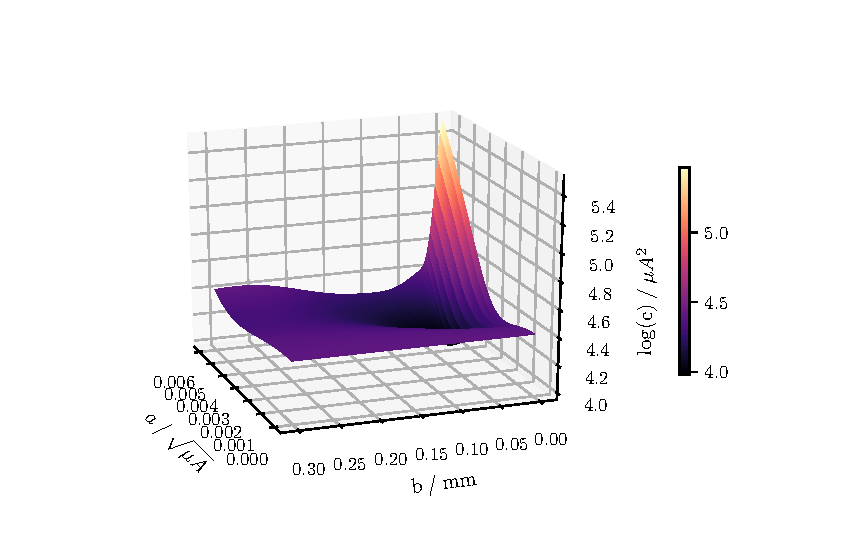
\includegraphics[width=.9\textwidth]{python/leastSquaresDoppel3ss.pdf}
    \caption{$s = \SI{0.75}{\milli\meter}$ (Herstellerangabe), $a = (0.00001, 0.006)$, $b = (0.0001, 0.3)$.}
    \label{fig:lsd3ss}
\end{figure}
\begin{figure}
    \centering
    \textbf{Parameterebene Doppelspalt - bester Fit, dynamische Parameter, kleine Intervalle}\par\medskip
    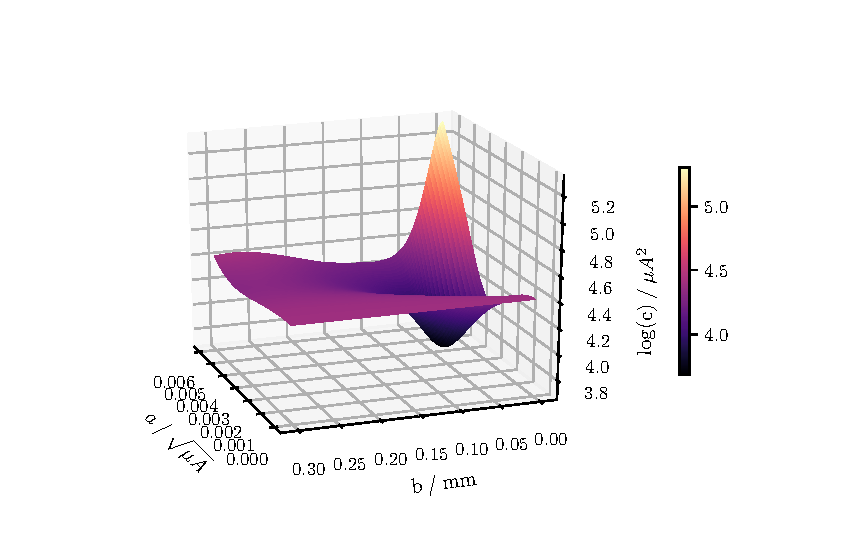
\includegraphics[width=.9\textwidth]{python/leastSquaresDoppel3s.pdf}
    \caption{$s = \SI{0.022}{\milli\meter}$, $a = (0.00001, 0.006)$, $b = (0.0001, 0.3)$.}
    \label{fig:lsd3s}
\end{figure}

Zum Vergleich werden zwei Ausgleichskurven mit entsprechenden Parameterwerten gegenübergestellt. Dabei wird je ein Parameter als Herstellerangabe
festgehalten und die nächstbeste Kurve berechnet.

\begin{figure}
    \centering
    \begin{subfigure}{.5\textwidth}
        \centering
        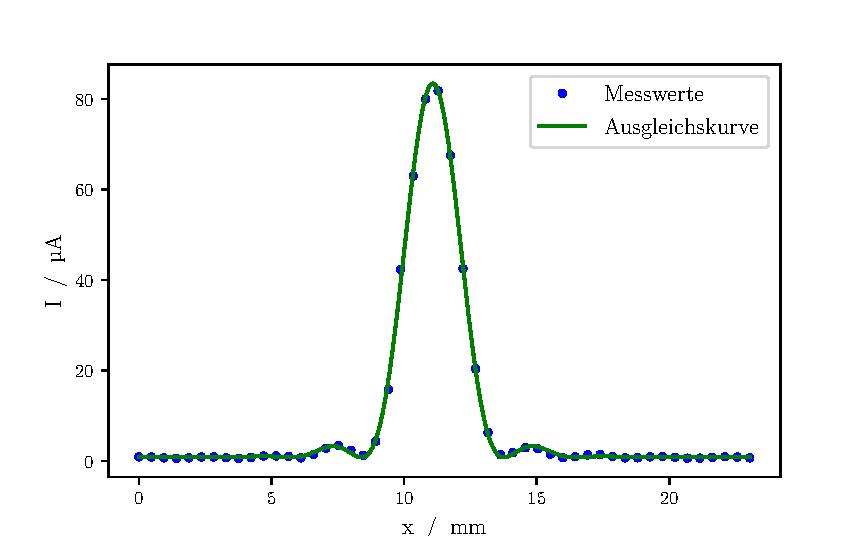
\includegraphics[width=.7\textwidth]{python/DoppelspaltFit.pdf}
        \caption{$s \approx \SI{0.022}{\milli\meter}$ mit $a \approx 0.005$, $b \approx 0.147$.}
        \label{fig:lsd3ss}
    \end{subfigure}%
    \begin{subfigure}{.5\textwidth}
        \centering
        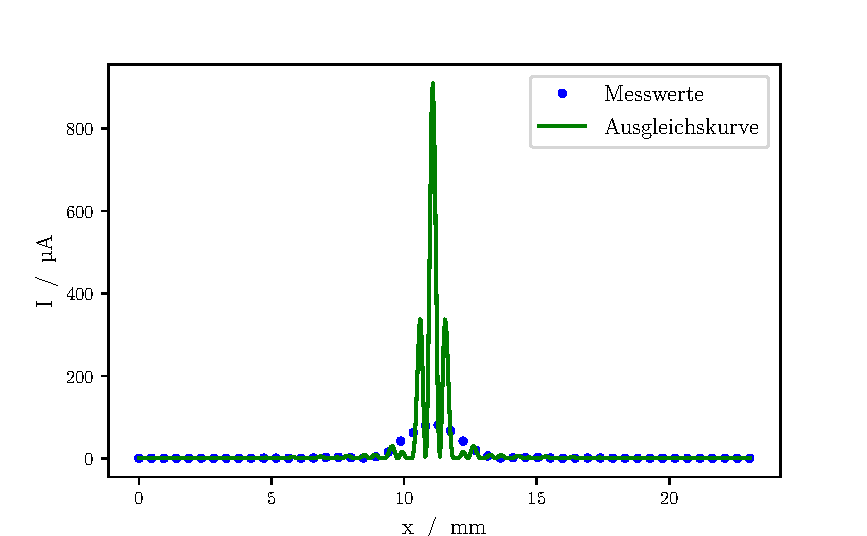
\includegraphics[width=.7\linewidth]{python/DoppelspaltFits.pdf}
        \caption{$s = \SI{0.75}{\milli\meter}$ mit $a \approx 0.015$, $b \approx 0.13$}.
        \label{fig:lsd3s}
    \end{subfigure}
    \caption{Doppelspalt nach \texttt{curve\_fit} (vgl. Tabelle \ref{tab:parDoppel}) vs. $s = \SI{0.75}{\milli\meter}$. Für alle: $x_0 = 11.077$, $I_d = 0.82$.}
        \label{fig:ggn1}
\end{figure}